\chapter{Design}
\label{sec:design}

% Ist das zentrale Kapitel der Arbeit. Hier werden das Ziel sowie die
% eigenen Ideen, Wertungen, Entwurfsentscheidungen vorgebracht. Es kann
% sich lohnen, verschiedene Möglichkeiten durchzuspielen und dann
% explizit zu begründen, warum man sich für eine bestimmte entschieden
% hat. Dieses Kapitel sollte - zumindest in Stichworten - schon bei den
% ersten Festlegungen eines Entwurfs skizziert werden.
% Es wird sich aber in einer normal verlaufenden
% Arbeit dauernd etwas daran ändern. Das Kapitel darf nicht zu
% detailliert werden, sonst langweilt sich der Leser. Es ist sehr
% wichtig, das richtige Abstraktionsniveau zu finden. Beim Verfassen
% sollte man auf die Wiederverwendbarkeit des Textes achten.

% Plant man eine Veröffentlichung aus der Arbeit zu machen, können von
% diesem Kapitel Teile genommen werden. Das Kapitel wird in der Regel
% wohl mindestens 8 Seiten haben, mehr als 20 können ein Hinweis darauf
% sein, daß das Abstraktionsniveau verfehlt wurde.

%%%%%%%%%%%%%%%%%%%%%%%%%%%%%%%%%%%%%%%%%%%%%%%%%%%%%%%%%%%%%%%%%%%%%%%%%%%%%%%%
%                                                                              %
% MOTIVATION                                                                   %
%                                                                              %
%%%%%%%%%%%%%%%%%%%%%%%%%%%%%%%%%%%%%%%%%%%%%%%%%%%%%%%%%%%%%%%%%%%%%%%%%%%%%%%%
\section{Motivation}

  Parallel computers are stricly necessary in scientific community
  where time to solution and the computation of big simulations
  is important. 

  \sitem { Simulations do not fit on a single node }
  \sitem { Simulation need to be distributed }
  \sitem { Distributed parts need to communicated }

  Assume, a parallel computer, a compute clusters (Section
  \ref{sec:cluster}), with a very homogeneous vertical and horizontal
  layout is used, in which the nodes are connected by a abitrary
  network and a simulation application is executed on the avaible
  ressources of this cluster. Usually, the simulation domain is
  decomposed (Section \ref{sec:domain_decomposition}) by a fixed
  algorithm in smaller chunks of work, subdomains, and then mapped
  onto the homogenous network of nodes on the cluster. So to speak a
  simulation domain is mapped one-to-one onto a
  homogeneous compute architecture. 

  \todo{Graphic one-to-one mapping}

  Simulation subdomains then communicate through predefined paths with
  each other to exchange simulation data. In concrete terms of MPI,
  that would mean,that MPI processes do communicate with a fixed set
  of other MPI processes by fixed communication operations defined by
  the simulation algorithm.

  This is the state of the art of the most simulations computed on
  cluster systems. And it is fine as long everything, both hardware
  and simulation, stay in this fixed relationship. Thus, there is no
  change necessary as long as a simulation will always be
  executed on the same cluster, with the same network topology
  and the same algorithms describing the simulation model. 

  But it is not possible to put all modern simulations in this box of
  a homogeneous world, because simulation applications have also
  heterogeneous behavior.  In vertical direction: multi scale effects,
  each representing a specific algorithm, are leading to varying
  communication topologies between subdomains and every communication
  topology usually require a sophisticated programming, that can be
  quite time costly.  In horizontal direction: subdomains have varying
  workload development over simulatin time. What does mean, that
  sooner or later the simulation runs into an unbalanced state of
  workload distribution. That unbalanced state does nor make use of
  all available compute ressource neither reduces simulation time to
  its minimum. Further, could a globally increased workload require a
  redistribution of the simulaton domain onto the available compute
  ressources.

  Not only the simulation domain can behave heterogeneous, but also
  the cluster hardware on which the simulation is executed. Thus,
  vertical cluster heterogenity is the developement of cluster nodes
  to multi socket, multi core and additional accelerator hardware,
  where each of this compute devices has its own hierarchical memory
  stucture, which need to be programmed with caution and knowledge
  about the device to really obtaine performance.  Also horizontal
  differences of cluster nodes are visible. Such that, a cluster can
  consist of varying node types for different task in the simulation
  application. Therfore, the simulation domain can not be mapped
  one-to-one on such a cluster configuration, but rather the mapping
  should be configurable explicitly.

  \todo{Graphic explicit mapping of simulation domain onto heterogeneous hardware}

  A real world example for such heterogeneous behavior of simulations
  is the PIConGPU simulation (Section \ref{sec:picongpu}). While
  magnetic and eletric fields only influence its direct neighboring
  fields, which requires next neighbor communication, particles
  interact globally with each other, which require an all to all
  communication algorithm. Furthermore, particles can move during
  simulation time to other subdomains, which leads to an unbalanced
  distribution of particles over the whole simulation domain. On the
  hardware side, PIConGPU is developed for the execution on cluster
  systems with NVIDIA accelerator hardware.  CPUs are respsonsible for
  data offload and communication over the network, some accelerators
  compute the simulation progress and others generate a vizualization
  of the simulated data. Thus, vertical and horizontal heterogenity
  both in simulation domain and on hardware cluster have already
  arrived in real world simulation applications.

  Actually, the state of the art communication libraries are not able to
  be adapted onto the needs of modern simulation applications.
  Therefore, there should be a intermediate layer between simulation
  application and compute cluster. This layer should allow a explicit
  mapping of the simulation domain onto the communication library,
  while the library should be easily exchangeable. Such that, the
  mapping can be adjusted onto heterogeneous behavior of simulation
  application and cluster hardware.

  \sitem { Solve load balancing problem }
  \sitem { Solve Fault tolerance problem }

  It was designed an approach for a flexible mapping of communication
  processes onto abitrary communication libraries. This design will
  be presented in the following sections. First of all the
  requirements for such a system is discussed. It follows a
  description of the overall design and then the design each component
  is discussed in datail.


%%%%%%%%%%%%%%%%%%%%%%%%%%%%%%%%%%%%%%%%%%%%%%%%%%%%%%%%%%%%%%%%%%%%%%%%%%%%%%%%
%                                                                              %
% REQUIREMENTS                                                                 %
%                                                                              %
%%%%%%%%%%%%%%%%%%%%%%%%%%%%%%%%%%%%%%%%%%%%%%%%%%%%%%%%%%%%%%%%%%%%%%%%%%%%%%%%
\subsection{Requirements}
\label{sec:requirements}


\begin{itemize}
\item Previous section described the state of the art of simulations on cluster systems and the problems of modern simulations
\item An intermediate layer is required
\item Layer should fullfill requirements
\item Simulation domain and subdomain can be quite varying
\item Algorithms on this domains also varying
\item Communication topology required by algorithm also varying
\item 3D Torus, N dimensional Grid, periodic boundary
\item Need possibility to describe and model communication topology very general
\item Communication not restricted to a single communication library
\item Flexible mapping from modeled communication topology onto existing communication library
\item The modeled communication topology and the abstraction from communication libraries
  form a virtual data exchange topology for algorithms
\end{itemize}

Summarising the described requirements results in the
following requirements of the system:

\begin{itemize}
\item Abstract data transfer method
\item Description of the communication topology
\item Virtual data exchange topology for algorithms
\item Mapping of communiation topology onto the hardware topology
\end{itemize}

%%%%%%%%%%%%%%%%%%%%%%%%%%%%%%%%%%%%%%%%%%%%%%%%%%%%%%%%%%%%%%%%%%%%%%%%%%%%%%%%
%                                                                              %
% ANALYSIS OF PIConGPU CODE                                                    %
%                                                                              %
%%%%%%%%%%%%%%%%%%%%%%%%%%%%%%%%%%%%%%%%%%%%%%%%%%%%%%%%%%%%%%%%%%%%%%%%%%%%%%%%
\section{Analysis of PIConGPU-Code}
\label{sec:picongpu_analysis}

The analysis of the PIConGPU source code and modeled simulation domain
plays as significant role in the design of the developed system.


\begin{itemize}
\item How does the communication topology looks like ?
  \begin{itemize}
  \item domain is divided into a 3-dimensional grid of cells
  \item two different types of effects : particles and fields
  \item fields do next neighbor communication 
  \item particles need all to all communication
  \end{itemize}
   


  \item What kind of communcation layer is used ?
    \begin{itemize}
      \item Communication is based on MPI and CUDA memcpy
      \item MPI used for communication over subdomain borders (p2p and collective)
      \item CUDA memcpy used for offload of simulation data from 
        host cpu to accelerator device and vice versa
    \end{itemize}

  \item How is Communication implemented in PIConGPU ?
    \begin{itemize}
      \item simulation data is stored in gridbuffer
      \item gridbuffer does automatically offload to accelerator
      \item gridbuffer knows its neighbor gridbuffers which
        are calculated by a function
      \item Communication operations are handled by a communicator class
      \item Collective operations are directly implemented by
        MPI collectives
    \end{itemize}

\end{itemize}


%%%%%%%%%%%%%%%%%%%%%%%%%%%%%%%%%%%%%%%%%%%%%%%%%%%%%%%%%%%%%%%%%%%%%%%%%%%%%%%%
%                                                                              %
% THE SYSTEM                                                                   %
%                                                                              %
%%%%%%%%%%%%%%%%%%%%%%%%%%%%%%%%%%%%%%%%%%%%%%%%%%%%%%%%%%%%%%%%%%%%%%%%%%%%%%%%
\section{Design of the System}

\todo{shortly describe state of the art system}

Due to the fact, that the communication hardware layout is fixed. The access
to the hardware is represented by CALs (See \ref{sec:cal}) and these
are connected in the simplest case by an fully connected network, thus
every peer can send messages to every other peer. Therefore a network
on top of the CALs has to be established.

It is a very important property to be able to explicitly map the
communication topology of the application onto the communication
hardware.

In the first place it should gives the application the possibility to
be optimized on special charakteristics of the compute cluster. For
example could vertices that need to communicate very intensively with
each other can be mapped on neighboring nodes or even onto the same
node. Which makes communication more efficient.

Besides it should be possible to change the mapping of the
communication topology onto the communication hardware in
runtime. This is important when thinking of occuring unbalanced load
during the run of the application.

The communication is abstracted from the actual communication layer by
the CAL and the communicaiton topology is modeled with a graph and
then maped onto the CAL.

\todo{add graphic for full system}

This section present the design of a system that fulfils the previous
discussed requirements (Section \ref{sec:comm_abstraction}). Therfore, the
methods to exchange data are abstracted (Section \ref{sec:cal}). Then,
an approach to describe the communication topology is described
(Section \ref{sec:graph}) and finally a way to map the simulation
domain onto the physical domain is presented (\ref{sec:gvon}).


%%%%%%%%%%%%%%%%%%%%%%%%%%%%%%%%%%%%%%%%%%%%%%%%%%%%%%%%%%%%%%%%%%%%%%%%%%%%%%%%
%                                                                              %
% COMMUNICATION ABSTRACTION LAYER                                              %
%                                                                              %
%%%%%%%%%%%%%%%%%%%%%%%%%%%%%%%%%%%%%%%%%%%%%%%%%%%%%%%%%%%%%%%%%%%%%%%%%%%%%%%%
\section{Abstraction from Existing Communication Layers}
\label{sec:comm_abstraction}

% Motivation for communication abstraction
Simulation applications can be interconnected by vast variety of
communication libraries. Most simulations make use of exactly one
possible libarary, but this reduces the simulation to compute systems
supporting exactly the selected library. This section describes an
approach to fulfil the previously discussed requirement of
a abstract data transfer method.

\todo{insert graphic of state of the art communication}

Assume a simulation  implements its communication by sockets
. Running this simulation on a local desktop machine can be quite
inefficient, because communication based on sockets adds unnecesary
overhead in a local environment. Replacing the communication library
by a mechanism that maps communication operations to local copies of
data or a hand over of memory addresses, would make communication in
this simulation more efficient. But replacing one method for data
exchange by another is not the solution of the problem. Rather
varying communication libraries should by addressable by the same
communication interface to make the application portable.

Thus, the abstraction from
this existing communication librariy is a fundamental property for a
portable application.  Even though, that there are existing standards
for communication in cluster systems, the world of computer science is
subject to constant change. The possibility to exchange the underlying
layer without changing the interface to this layer, is a precondition
for future applications in distributed computing.

The challange is to provide a very general interface, that gives the
possibility to address varying communication libraries through it.
This interface should be as transparent as possible, such that it
reminds the interface user on his present communication library.  It
should be easily deployable into existing applications by replacing
the actual communication library without changing the fundamental
understanding of the way to communicate within this application.


%%%%%%%%%%%%%%%%%%%%%%%%%%%%%%%%%%%%%%%%%%%%%%%%%%%%%%%%%%%%%%%%%%%%%%%%%%%%%%%%
%                                                                              %
% CAL                                                                          %
%                                                                              %
%%%%%%%%%%%%%%%%%%%%%%%%%%%%%%%%%%%%%%%%%%%%%%%%%%%%%%%%%%%%%%%%%%%%%%%%%%%%%%%%
\subsection{Communication Abstraction Layer (CAL)}
\label{sec:cal}

\sitem{Instances participating on communication in general are called peers subsequently}

The \textit{Communication Abstraction Layer}, shortly \textit{CAL}, is
a generic communication interface on top of an existing communication
library. The libraries are addressable through adapters, which makes it
possible to address varying communication libraries . By exchanging
the adapter, the application based on the interface can be ported to
varying communication libraries without changing interface function
calls. The CAL is configured by an adapter at compile time, thus, by
using this flexible approach no runtime overhead should occur by using
the abstract interface instead of the original interface.

While the CAL provides an abstract interface with common communication
methods,  the adapter  implements the  interface demanded  by the  CAL
through library  its particular communication  operations. 

The  interface of
the  CAL provides  basic direct  communication operations,  collective
operations and  operation for  grouping of peers  Figure \ref{fig:cal}
shows  the   communication  abstraction  layer  on   top  of  existing
communication layers.  The CAL with  a specific adatper  could already
replace a  specific communication library in  simulation applications,
but the it is not meant to be the level of abstraction the simulation
programmer will interact  with. Further layers of  abstraction will be
discussed in later sections \ref{sec:graph} and \ref{sec:gvon}.

\begin{figure}[H]
  \centering 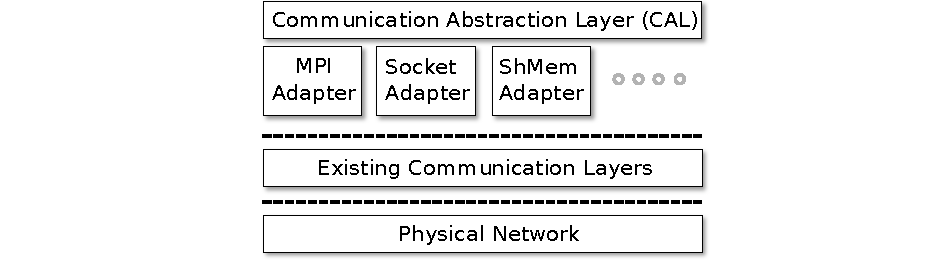
\includegraphics[width=\textwidth]{graphics/30_cal}
  \caption{A part of the design with Communication Abstraction Layer
    (CAL) on top of existing communication layers. Varying libraies
    can be addressed through the CAL interface, when an according
    adapter for this library is implemented.}
  \label{fig:cal}
\end{figure}

Thus, Using the CAL instead of a concrete communication library has
the advantage that changing communication environment, by migrating to
another compute architecture, only the adapter has to be exchanged,
the application has to be recompiled, but the CAL interface stays the
same.


%%%%%%%%%%%%%%%%%%%%%%%%%%%%%%%%%%%%%%%%%%%%%%%%%%%%%%%%%%%%%%%%%%%%%%%%%%%%%%%%
%                                                                              %
% ADDRESSING OF PEERS                                                          %
%                                                                              %
%%%%%%%%%%%%%%%%%%%%%%%%%%%%%%%%%%%%%%%%%%%%%%%%%%%%%%%%%%%%%%%%%%%%%%%%%%%%%%%%
\subsection{Addressing of Peers}
% CAL virtual addressing
Each communication library comes with its own way to address peers,
which can be quiete different. Socket based systems address their
peers by ip addresses, MPI based systems address their processes by
ranks and systems based on memory copies are using memory addresses.
These diverse approaches to address peers in a network need to be
translated to an unified address space to provide a unified interface of the CAL.
Therefore, a CAL provides a virtual address which is an unique
identifier for its peer. The virtual address
will be abbreviated in some points by vaddr. Based on this virtual
address, peers are able to address each other through the CAL
interface.

The translation of virtual addresses to the adapter specific real address
is resolved by the adapter itself. Thus, the adapter defines how the participants
of its network are mapped onto the given virtual address space of the CAL. This
mapping is invisible for the CAL, so that the CAL only handle virtual addresses
and the adapter handles its particular address space.


%%%%%%%%%%%%%%%%%%%%%%%%%%%%%%%%%%%%%%%%%%%%%%%%%%%%%%%%%%%%%%%%%%%%%%%%%%%%%%%%
%                                                                              %
% MULTI ADAPTER                                                                %
%                                                                              %
%%%%%%%%%%%%%%%%%%%%%%%%%%%%%%%%%%%%%%%%%%%%%%%%%%%%%%%%%%%%%%%%%%%%%%%%%%%%%%%%
\subsection{Multiadapter}

The possibility to exchange the adapter of the CAL also raises the
question if a design with more than one adapter at the same time would
be possible. Connecting the network of at least two adapters would
form a heterogeneous network, where each network has its own
properties like latency, bandwidth and hardware topology. The CAL
would unify these varying networks under the same interface. Thus, a
multi adapter design is the foundation for the usage of the developed
system in jungle computing environments
\ref{sec:jungle}.

Assume, the CAL has two adapters, one for MPI and another for sockets,
to chose from and some peers of the network are able to communicate
through both adapters.  The CAL needs to provide a list of all
avaiblabe adapters for a specific peer. A particular sorting of this
list could state out the prefered adapter for communication between
two peers. Exchanging data between peers always requires a lookup of
which adapter needs to be selected to address the peers.

\sitem{strategy patter}
\sitem{variadic templates}

Furthermore, varying real addresses spaces of different adapters have
to be mapped onto the same unified address space of the CAL.
It opens up the possibility that two peers which do not share a same
adapter, but are connected over a third adapter, could still exchange data
by routing over that third adapter. Thus, a multi adapter design
does only make sense when routing between two adapters is implemented.

\sitem{Connecting cluster systems over internet}
\sitem{Easily create grid computing structures}

Even if the design of a multi adapter communication abstraction layer
looks quite interesting, the implementation is rather more komplex
than a single adapter design. 

It is not planed in the actual design that the CAL provides routing
abilities. Peers have to be connected directly by the network of the
adapter. No routing makes it also impossible to forward data between
different adapters of the CAL. Thus a specific CAL only provides a
single adapter. But several CALs can be used with different adapters
to communcate on several networks. In such a scenario the routing can
be implemented on top of the CAL by the library user. Therefore, the
design was first pushed forward in the direction of a single adapter
design and a multi adapter design is left open for future work.


%%%%%%%%%%%%%%%%%%%%%%%%%%%%%%%%%%%%%%%%%%%%%%%%%%%%%%%%%%%%%%%%%%%%%%%%%%%%%%%%
%                                                                              %
% CAL INTERFACE                                                                %
%                                                                              %
%%%%%%%%%%%%%%%%%%%%%%%%%%%%%%%%%%%%%%%%%%%%%%%%%%%%%%%%%%%%%%%%%%%%%%%%%%%%%%%%
\subsection{Communication Interface}
\label{sec:cal_comm}
% Peer2Peer Operations
\subsubsection{Peer to Peer Operations}

In the first place, the CAL provides peer-to-peer communication. That
are basic communication methods to exchange abitrary data between two
peers, like sending and receiving.  These operations are available
both blocking and non-blocking.

\sitem{Non-blocking operations return an event}
\sitem{Events representing the state of the previously executed communication operation}
\sitem{Operation is either still processing or has already finished}
\sitem{Event provides a method to query the present state}
\sitem{Event provides function to wait for the operation until it has finished}
\sitem{CAL defines event interface}
\sitem{Event is very adapter specific}
\sitem{Each communication library treats non blocking communication differently}
\sitem{Event need to be implemented by the adapter}

A direct communication operation is called with a triplet of
arguments, including the virtual address of sender or receiver, the
message description tag and the actual data to exchange.  The
interface is influenced by existing communication libraries that all
share a common interface \cite{ref:boost_mpi, ref:boost_asio,
  ref:zmq}.The message description tag is a simple header of the
message. It helps to easily distinguish between messages of the same
sending peer.  The data object should provide methods to retrieve the
data pointer and the size of the data. The data pointer should point
to a contigiuous memory area. The following list describes the
direction communication operations of the CAL interface:

\begin{itemize}
  \item void send(destination vaddr, tag, data)
  \item void recv(source vaddr, tag, data)
  \item Event asyncSend(destination vaddr, tag, data)
  \item Event asyncSecv(source vaddr, tag, data)
\end{itemize}


%%%%%%%%%%%%%%%%%%%%%%%%%%%%%%%%%%%%%%%%%%%%%%%%%%%%%%%%%%%%%%%%%%%%%%%%%%%%%%%%
%                                                                              %
% CONTEXT                                                                      %
%                                                                              %
%%%%%%%%%%%%%%%%%%%%%%%%%%%%%%%%%%%%%%%%%%%%%%%%%%%%%%%%%%%%%%%%%%%%%%%%%%%%%%%%
\subsubsection{Grouping of peers}
\label{sec:cal_context}
Grouping of peers is, next to the communication methods, the most
important function the CAL provides by its interface.  By default, all
peers of the CAL are grouped to a global group of peers.  A group of
peers will be called \textit{context}. Such that, the global group is
called global context.

A context stores the information about the peers virtual address , the
amount of peers grouped and whether the context is valid for that
peer. It is the base for communication algorithms with more than 2
participating peers. These algorithm are introduced as collective
operations (Section \ref{sec:collectives}).

The CAl provides always the global context of which a peer
can retrieve its global virtual address. A new context can
be created from a subset of peers of an already existing
context. Thus, a new context can be creates by the
requirements of the communication algorithm. This new context
provides its own virtual address space, thus, the virtual
address of a peer is context dependent.

Managing of contexts can be quiete adapter specific. Thus, the CAL
only defines the context interface, but an adapter needs to implement
a context for its particualar communication library. Furhtermore, the
adapter has to mind that a virtual address is context dependent, such
that the mapping of virtual address to real address has to be adapted
to varying contexts.

%%%%%%%%%%%%%%%%%%%%%%%%%%%%%%%%%%%%%%%%%%%%%%%%%%%%%%%%%%%%%%%%%%%%%%%%%%%%%%%%
%                                                                              %
% COLLECTIVE OPERATIONS                                                        %
%                                                                              %
%%%%%%%%%%%%%%%%%%%%%%%%%%%%%%%%%%%%%%%%%%%%%%%%%%%%%%%%%%%%%%%%%%%%%%%%%%%%%%%%
\subsubsection{Collective Operations}
\label{sec:cal_collective}
A \textit{collective operation}, short \textit{collective}, is a
communication pattern, that is executed simultaneously by all peers of
a context. Collectives are used to collect, distribute, share and
reduce data.  Each collective can be implemented by a sequence of peer
to peer operations, but communication libraries, especially the ones for
high performance calculations, often come with optimized collective support.

A Collective is always executed in respect to a context and the result
is either received by only one peer, the root, or by all peers.  While
a large number of collectives is known to the parallel computation
commmunity, the CAL only provides the most common ones with respect to
the analysis of the PIConGPU source code (Section \ref{sec:picongpu_analysis}).

The following is a list of all provided collective operations of the
CAL and its description:
\begin{itemize}
\item gather(root, context, send, recv)\\

  Collection of data elements from every peer in the context. Each peer
  contributes the same number of data elements. The collected data will
  be received from the root peer.

\item allGather(context, send, recv)\\

  A gather collective, while all peers of the context receive the data.

\item scatter(root, context, send, recv)\\

  Distribution of data elements from the root peer to all other peers of
  the context. The data will be divided into chunks of same
  size. Assuming the number of data elements is divisible by the number
  of peers, every peer will receive the same number of data
  elements. Thus, every peer receives different data elements.

\item allScatter(context, send, recv)\\

  A scatter collective, while all peers of the context receive the data.

\item reduce(root, context, operation, send, recv)\\

  Reduction of the data elements from every peer of a context by a
  binary function. A binary function, takes two arguments of abitrary
  type and returns a value of abitrary type. Usually both input
  arguments and return value have the same type.

\item allReduce(context, operation, send, recv)\\

  A reduce collective, while all peers of the context receive the
  data.

\item void broadcast(root, context, data)\\

  Distributes data elements from the root peer to all other peers of
  the context. Every peer receives the same data elements.

\item syncronize(context)\\

  This operation synchronizes the control flow of all peers of the
  context.

\item createContext(peers, context)\\ 

  Creation of a new context from a subset of peers of an already
  present context.

\end{itemize}

The listed collectives have all homogeneous behavior. All peers either
send the same amount of data or receive the same number of data elements.
Some algorithms require an  exchange of varying number of data elements. Thus,
collectives like gather, allGather, scatter, allScatter are also available
in a variant with varying number of data elements per peer. These collectives
get an additional receive count argument, that describes how many data elements
each peer has contributed to the collective.


%%%%%%%%%%%%%%%%%%%%%%%%%%%%%%%%%%%%%%%%%%%%%%%%%%%%%%%%%%%%%%%%%%%%%%%%%%%%%%%%
%                                                                              %
% GRAPH                                                                        %
%                                                                              %
%%%%%%%%%%%%%%%%%%%%%%%%%%%%%%%%%%%%%%%%%%%%%%%%%%%%%%%%%%%%%%%%%%%%%%%%%%%%%%%%
\section{Modeling of the Application Domain}
\label{sec:graph}
The simulation application always implements a particular algorithm
that describes a particular model. This Algorithm often requires a
domain decomposition (Section \ref{sec:domain_decomposition} of the
simulation domain into a set of subdomains. Assume, subdomains need
to interact with each other, communication between subdomains is
necessary. Thus, the choosen algorithm of the simulation determines
the communication topology .

The communication and its underlying communication topology is often
implemented in a implicit and static manner. The simulation domain is
mapped fixed onto the compute ressources.  Such that, a change of the
simulation algorithm need to be translated into a change of the
coresponding communication patterns, which can be quiete costly.

A more elegant approach is to explicitly model the relationships
between the subdomains and therefore the communication topology. The
most general method to model a topology is a \textit{graph}
\cite{ref:graph}.  From a mathematical perspective, a graph is a pair
of vertices and edges. Edges are pairs of vertices. So to speak, a
graph represents a set of objects, where some of these objects are
connected by links.

Changing the simulation domain implies a different communication
topology and in turn implies a different graph.  Since, the
communication topology is explicit modeld by a graph, it is not
necessary to rewrite the simulation application as long the
application is oriented on the topology information provided by the
graph. Thus, algorithms can by implemented on top of the graph
description.

% directed cycle multi graph

The graph has the property, that vertices are connected by directed edges. Loops
and multiple edges between two vertices are allowed (Figure
\ref{fig:graph}). The resulting graph is a directed multi graph with
loops. The mathematical expression for this kind of graph is quiver
\cite{ref:quiver}

\begin{figure}[H]
  \centering 
\includegraphics[width=\textwidth]{graphics/30_graph}
  \caption{ A directed cycle multi graph with vertices A, B and edges
    1, 2, 3.  }
  \label{fig:graph}
\end{figure}
\todo{Bigger, better looking graph}

\sitem{Graph provides methods to retrieve information from it}
\sitem{All vertices or specific vertex}
\sitem{Adjacent vertices of a vertex}
\sitem{Out edges of a vertex}
\sitem{In edges of a vertex}
\sitem{Creation of subgraphs}

%%%%%%%%%%%%%%%%%%%%%%%%%%%%%%%%%%%%%%%%%%%%%%%%%%%%%%%%%%%%%%%%%%%%%%%%%%%%%%%%
%                                                                              %
% GRAPH PROPERTIES                                                             %
%                                                                              %
%%%%%%%%%%%%%%%%%%%%%%%%%%%%%%%%%%%%%%%%%%%%%%%%%%%%%%%%%%%%%%%%%%%%%%%%%%%%%%%%
\subsection{Properties}
A graph alone is just the representation of connected vertices, but
has no connection to the simulation domain. The connection usually
only exists in the head of the programmer of the simulation
application. But, a graph can be interpreted as a container, wherby the
objects of the container are in a relation to each other.

The container object will be called property and is introduced as a
concpet to annotate a graph. A property provides subdomain information
and can be bound to vertices and edges (Figure
\ref{fig:property}). Vertices and Edges of the same graph share
respecively the same type of property. A graph annoted with properties
is significantly more meaningful and thus helps to keep the connection
of the simulation domain and communication topology.

\begin{figure}[H]
  \centering 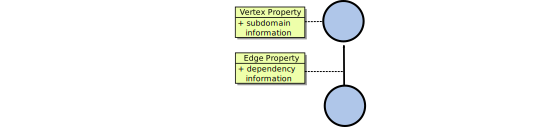
\includegraphics[width=\textwidth]{graphics/30_property}
  \caption{A graph with both vertex and edge properties. The vertex
    property primarily describe a subdomain. The edge property
    describe the dependencies between subdomains.}
  \label{fig:property}
\end{figure}

A Property can also be used to create a connection between a pair of
graphs. Thus a modeling of hiararchical domains is also possible.  A
later example will make use of this hierarchical modeling (Section
\ref{sec:gol}).

%%%%%%%%%%%%%%%%%%%%%%%%%%%%%%%%%%%%%%%%%%%%%%%%%%%%%%%%%%%%%%%%%%%%%%%%%%%%%%%%
%                                                                              %
% MODELING GAME OF LIFE AS A GRAPH                                             %
%                                                                              %
%%%%%%%%%%%%%%%%%%%%%%%%%%%%%%%%%%%%%%%%%%%%%%%%%%%%%%%%%%%%%%%%%%%%%%%%%%%%%%%%
\subsection{Modeling Game of Life as a graph}
\label{sec:gol}
To give an example for modeling a specific simulation application,
Figure \ref{fig:gol} models the Game of Life (GoL) \cite{ref:gol}
domain by a graph. GoL simulates the evolution of a set of cells for
an abitrary amount of timesteps. The cells are arranged in a two-
dimensional grid.  A cell has a state which is either alive or not
alive and the state of the next time step is calculated by
rules. The common set of rules determine the state of a cell for the
next time step by the state information of the neighboring cells. One
rule for example is, that a dead cell with exactly 3 living cells in
the neighborhood will be reborn on the next time step. For the further
description of GoL it is assumed the only this rule exists.

\todo{Game of life description graphic from status presentation}

Modeling this common rule straight forward, ending up in a graph where
every cell of the GoL world is represented by a vertex and neighboring
cells are connected by an edge. Each vertex has the property cell, that
contains the state of the cell. Figure \ref{fig:gol} shows a vizualized
cut out of the GoL modeled domain. To determine the next state of a 
cell, it has to count the living adjacent cells in the graph and if
exactly three adjacent cells are alive, then the cell will also be
alive on the next time step.

\begin{figure}[H]
  \centering 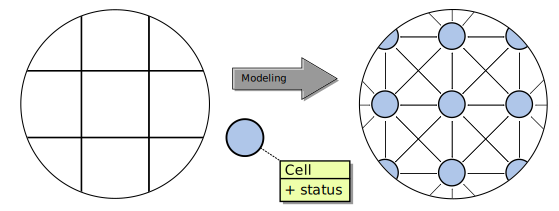
\includegraphics[width=\textwidth]{graphics/30_gol}
  \caption{Cut-out of a Game of Life domain (on the left) was modeled
    as a graph (on the right). Each Vertex is described by the vertex
    property cell, containing the state information of the cell. A
    Vertex determines next state by state of neighboring cells}
  \label{fig:gol}
\end{figure}

Now changing the rule slightly to a GoL where a cell needs some free
area around itself, thus, a cell can be only alive if the living cells
in the neighborhood have a distance of one cell that is not
alive. This changes the GoL communication topology and therefore the
graph, so that cells are not only connected to its next neighbors, but
also to its next next neighbors. Nonetheless, to determine the next
state of a cell, it has to count the living cells of next and next
next neighbors.

\todo{Graph for changed rule}

% Partitioned graph
The graph in figure \ref{fig:gol} models the GoL domain very fine
granular by every individual cell. While it is the smallest possible
domain decomposition, it might not be very efficient when this graph
is the foundation for a distributed computing application. Imagining, a
single cell is calculated by a process and the cell state is exchanged
by inter-process communication, but single process can compute
considerably more cells.

\sitem{Adding a further graph to the GoL modeling}

Figure \ref{fig:gol_bundle} shows the partioning of the fine granular
GoL graph by bundling multiple vertices together to a partioned
graph. A parition of vertices is called a bundle. These Bundles are
connected by edges when at least one cell on the border of a bundle
is the neighbor of a border cell from another bundle.  The creation of
a partioned graph by bundles with a minimum of connections is the
topic graph partitioning algorithms. But the modeling of an optimal
partitioned graph is not part of this work.

While the fine granular GoL graph represents the GoL cells in detail, the
partitioned graph represents dependencies of bundled cells. Thus
the properties of the partioned graph changed such that bundles
have store the cells they bundle and edges refer to neighboring
cells.

\begin{figure}[H]
  \centering 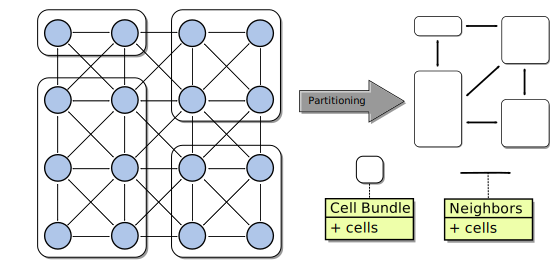
\includegraphics[width=\textwidth]{graphics/30_gol_bundle}
  \caption{The GoL graph is partitioned by bundling multiple
    cells. The properties of the partioned graph have changed, such
    that the vertex property contains the cells of a bundle, while the
    edge property contains information about neighboring cells.}
  \label{fig:gol_bundle}
\end{figure}

The partitioned graph could be used as foundation to distribute GoL to
multiple devices on a cluster. Each bundle could be computed by an own
process. The Processes do calculation for their local GoL graph and
communicate states of their border cells to adjacent bundles.

\sitem{It has been shown a different approach to model game of life}
\sitem{Used the same description tool; the graph}
\sitem{Both graph were connected over its graph properties}


%%%%%%%%%%%%%%%%%%%%%%%%%%%%%%%%%%%%%%%%%%%%%%%%%%%%%%%%%%%%%%%%%%%%%%%%%%%%%%%%
%                                                                              %
% GRAPH-BASED VIRTUAL OVERLAY NETWORK (GVON)                                   %
%                                                                              %
%%%%%%%%%%%%%%%%%%%%%%%%%%%%%%%%%%%%%%%%%%%%%%%%%%%%%%%%%%%%%%%%%%%%%%%%%%%%%%%%
\section{Graph-Based Virtual Overlay Network (GVON)}
\label{sec:gvon}
The previous sections described the tools to communicate and to
model the communication topology. By providing an explicit mapping of
the communication topology onto the abstract communication layer,
the combination of these tools establish a virtual communication layer
within the simulation domain.  Such that, communication between
subdomains of the application can be represented. Therefore, this
section introduces a \textit{graph-based virtual overlay network},
short GVON, that is based on the graphs and the CAL.

The graph does provide a simulation domain specific communication topology.  It is
used as a blueprint for the virtual network topology.  Communication
operations are provided by the CAL as base for the overlay network.
Figure \ref{fig:gvon} shows the GVON as a layer between the graph and
CAL on one side and the application on the other side.

\begin{figure}[H]
  \centering 
\includegraphics[width=\textwidth]{graphics/30_gvon}
  \caption{The graph-based virtual overlay network provides
    communication functionality based on the CAL, but uses the
    communication topology modeled by the graph.}
  \label{fig:gvon}
\end{figure}

All peers that want to take part on the communication of the GVON need
to know exactly the same graph. In order to ensure that, the graph can be
constructed in parallel by all peers, loaded from the same file of a
distributed file system or could even be delivered by a master
peer. Furthermore, peers need to use the same adapter configuring its
CAL, otherwise a communication is not possible.


%%%%%%%%%%%%%%%%%%%%%%%%%%%%%%%%%%%%%%%%%%%%%%%%%%%%%%%%%%%%%%%%%%%%%%%%%%%%%%%%
%                                                                              %
% GVON MAPPING                                                                 %
%                                                                              %
%%%%%%%%%%%%%%%%%%%%%%%%%%%%%%%%%%%%%%%%%%%%%%%%%%%%%%%%%%%%%%%%%%%%%%%%%%%%%%%%
\subsection{Mapping of the graph onto the CAL}
\label{sec:mapping}
The connection between a graph and a CAL is a mapping of vertices to
peers, called the vertex map.  A vertex map is valid for a particular
graph. The GVON provides for a another graph, another vertex map.  The
mapping of vertices to peers is a joint process of all peers that want
participate in the communication based on a particular graph.

The first phase is the distribution of the vertices of the graph to
the peers (Figure \ref{fig:gvon_mapping}), where every peer gets
assigned a set of vertices. There are a varity of methods to
distribute the vertices.  It could be done totally randomized, round
robin or even dictated by some master peer. The distribution behavior
is defined by the user of the developed system and might be object for
further optimization, but it was not topic of this work to find optimal
distributions.

\begin{figure}[H]
  \centering 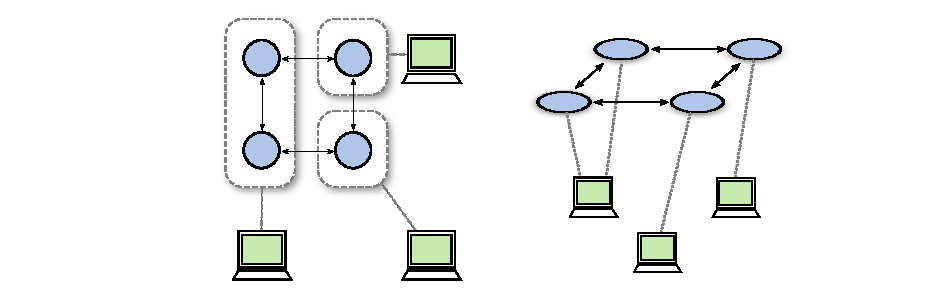
\includegraphics[width=\textwidth]{graphics/30_gon_mapping}
  \caption{All vertices of a graph are distributed onto 3 peers. The vertices
  are not distributed evenly, thus one peer is host for 2 vertices.}
  \label{fig:gvon_mapping}
\end{figure}

In the next phase the peers announce their vertices to all other
peers.  A peer that announces vertices is called host and the
announced vertices are called hosted vertices.  Every host receives
from every other host a list of its hosted vertices and stores this
information in its vertex map. A host is responsible for the
communication of its hosted vertices. A host is responsible either for
zero, one or more vertices. So to speak, it is also possible that host
is responsible for all vertices of a graph and communicates finally
always with itself.  Depending on the used adapter this might not even
be a problem, since communication of a peer with itself can be mapped
to local memory copies and does not necessarily go over the network.

Furthermore the GVON provides a mapping of the graph of the announced
vertices to a context (Section \ref{sec:cal_context}), called the
graph map. This mapping is necessary since the GVON will also be used
to map collective operations on the graphs onto the CAL.

The vertex and graph map is the basis for the mapping of communication
processes onto the hardware.


%%%%%%%%%%%%%%%%%%%%%%%%%%%%%%%%%%%%%%%%%%%%%%%%%%%%%%%%%%%%%%%%%%%%%%%%%%%%%%%%
%                                                                              %
% GVON COMMUNICATION                                                           %
%                                                                              %
%%%%%%%%%%%%%%%%%%%%%%%%%%%%%%%%%%%%%%%%%%%%%%%%%%%%%%%%%%%%%%%%%%%%%%%%%%%%%%%%
\subsection{Communication within the GVON}
In the context of an overlay network, a vertex is interpreted as a
virtual peer, edges between adjacent vertices indicate that the
virtual peers are able to communicate with each other. Thus, the
application on top of the GVON has the transparent view, that it is
really exchanging messages between the vertices and the GVON is taking
care, that the messages are reaching the correct vertex host. Thus, 
this level of abstraction is finally the level the application
interacts with.

The GVON provides similar functionality like the introduced
communication operations in the CAL, but on graph basis. Thus both
peer to peer and collective operations are provided.

% GVON P2P
A peer to peer operations within the GVON involves exchanging data
between adjacent vertices over a particular edge of a particular graph.

\sitem{Operations can by blocking or non blocking}
\sitem{Non blocking, returning an event}

The interface looks like the following:

\begin{itemize}
  \item void send(graph, destination vertex, edge, data)
  \item void recv(graph, source vertex, edge, data)
  \item Event asyncSend(graph, destination vertex, edge, data)
  \item Event asyncRecv(graph, source vertex, edge, data)
\end{itemize}

The GVON has the task to resolv both the context of a graph and the
host of the source or the destination vertex. This information are
quieried from the vertex and graph map. When this information is
resolved the programm flow is handed over to the CAL. The Cal is then
responsible for exchange data between the hosts.

% GVON collectives
Operations between all vertices of a graph can be performed as
collective operations (Section \ref{sec:collectives}). A host needs to
perform the collective operation for all its hosted vertices,
otherwise it blocks the execution of the operation. Yet again,
the result of the collective is received by some root vertex
or by all vertices of the graph.

\sitem{Collectives of the GVON are transparent to the application}

The collective operation is first executed locally for all hosted
vertices of each host. Then it is further handled by the CAL and
transmitted to the receiver(s). Figure \ref{fig:gvon_collective} shows
a gather operation on the same graph and mapping of figure
\ref{fig:gvon_mapping}. A gather operation collects the data of hosted
vertices of a host first locally and uses then the gather operation
provided by the CAL. A similar approach is used for the reduce
operation, whereby data is either collected or reduced locally to a
single value, depending on the commutativity of the reduce
operation. 

\sitem{synchronize only if for all hosted vertices of a host called}
\sitem{no real barrier, but simulates behaviour}

\sitem{Execution of collective could be done sequential or parallel}
\sitem{Both variants have their problems}
\sitem{sequential could lead to dead lock behaviour}
\sitem{programmer has to pay attention to call collecitve for every hosted vertex}

\begin{figure}[H]
  \centering 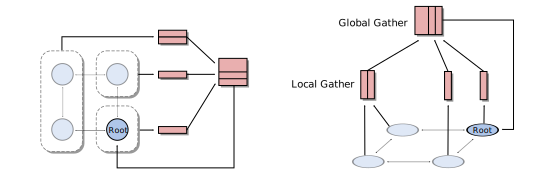
\includegraphics[width=\textwidth]{graphics/30_gon_collective}
  \caption{Gather operation with the GVON. Data is first locally 
    and then globally collected. Finally the collected data
    is transmitted to the root vertex.}
  \label{fig:gvon_collective}
\end{figure}


%%%%%%%%%%%%%%%%%%%%%%%%%%%%%%%%%%%%%%%%%%%%%%%%%%%%%%%%%%%%%%%%%%%%%%%%%%%%%%%%
%                                                                              %
% REMAPPING                                                                    %
%                                                                              %
%%%%%%%%%%%%%%%%%%%%%%%%%%%%%%%%%%%%%%%%%%%%%%%%%%%%%%%%%%%%%%%%%%%%%%%%%%%%%%%%
\subsection{Remapping of Vertices}
\label{sec:remapping}
Since, the communication topology is seperated from the communication
layer, it is possible to change the mapping from vertices to peers at
runtime. This runtime behavior is an interesting fact in respect to
load balancing and fault tolerance.

Load balancing can be an issue when the communication topology is
changing during simulation execution. For example could the GoL
simulation add a new rule, which leads to a changed communication
topology for that in turn exists a better vertex mapping. Even if the
performance of a cluster network link drops, thus, some peers are not
able reach accetable latency and bandwidth between each other, a
remapping could solve this problem at runtime.

\sitem{move of calculation load is also an issue for remapping}

Another issue is the failure of single cluster nodes and therefore
also a failure of hosts loacted on this nodes. Assuming, that the data
of hosts where backuped, for example through checkpointing techniques,
the hosted vertices of the failed host can be adopted by another host,
also at runtime.

The process of remapping is very similar to the mapping process of
section \ref{sec:mapping}.  It is also divided in two steps:
distribution and announcment. It has to be distinguished between
global and local remapping. A global remapping is a repetition of the
mapping process of section \ref{sec:mapping}. A local remapping does
not require a full redistribution of vertices.  Since the remapping
situation is slightly different, so that host already own a set of
hosted vertices, the distribution is more a swap or occupation of
vertices.

\todo{remapping figure, take it from the talk}

\cleardoublepage

%%% Local Variables:
%%% TeX-master: "diplom"
%%% End:
